\documentclass[10pt]{beamer}
\usetheme{Madrid}
\usecolortheme{whale}

\usepackage[utf8]{inputenc}
% \usepackage[french]{babel}
\usepackage{amsfonts}
\usepackage{booktabs}
\usepackage{graphicx}
\usepackage{tikz}
\usetikzlibrary{external}
\tikzexternalize % Crée un cache pour le graphe de la slide 10 (évite de le recalculer)
\usepackage{environ}
\setkeys{Gin}{draft=false} % Force le non chargement des images.


% --- Informations de la Soutenance ---
\title[Explicabilité et décorrélation dans les graphes]{Explicabilité additive et décorrélation structurelle dans les graphes complexes}
\subtitle{Soutenance de Stage de Fin d'Études}
\author[Guilhem DUPUY]{Guilhem DUPUY, encadré par Rémy CAZABET}
\institute[LIRIS - équipe DM2L]{Université Lyon 1, LIRIS - équipe DM2L}
\date{25 Juin 2026}

\begin{document}

% Slide 1 : Titre
\begin{frame}
    \titlepage
\end{frame}

% Slide 2 : Sommaire
\begin{frame}{Plan de la présentation}
    \tableofcontents
\end{frame}

\section{Introduction et Problématique}

% Slide 3 : Contexte des Réseaux Complexes
\begin{frame}{Contexte : L'analyse des réseaux complexes}
    \begin{itemize}
        \item \textbf{Modélisation par graphes :} représenter interractions entre entités (réseaux sociaux, infrastructures, biologie ...)
        \item \textbf{Forces structurantes sous-jacentes :} Multiples facteurs gouvernent la formation des liens.
        \begin{block}{1. Le paradigme communautaire}
            Présence de blocs/communautés d'affinité (ex. Modèles SBM). La connectivité dépend des groupes latents.
        \end{block}
        \begin{block}{2. Le paradigme géométrique}
            La probabilité de lien décroît avec la distance physique (ex. Modèles spatiaux gravitaires)
        \end{block}
    \end{itemize}
\end{frame}

% Slide 4 : La Prédiction de Liens comme Instrument
\begin{frame}{Problématique : la boîte noire de la prédiction de liens}
    \begin{block}{Le contexte : La prédiction de liens comme instrument}
        Utilisée comme outil pour mesurer la qualité d'une représentation de graphe.
        \begin{itemize}
            \item \textbf{Modèles performants :} Louvain, SBM, modèles d'espace latent, etc.
        \end{itemize}
    \end{block}

    \vspace{0.3cm}

    \begin{alertblock}{Le verrou scientifique : Une explicabilité limitée}
        Les approches d'explicabilité classiques sont \textbf{locales}, reposant sur des sous-graphes.
        Charge de l'interprétation pour l'utilisateur.
    \end{alertblock}

    \vspace{0.3cm}

    \begin{exampleblock}{Notre question de recherche :}
        \centering
        \smallskip
        \textbf{Comment décomposer et expliquer l'origine des liens comme une somme de différents facteurs (communautaires, géométriques, etc.) ?}
        \smallskip
    \end{exampleblock}
\end{frame}

% Slide 5 : Objectifs du Stage
\begin{frame}{Objectifs et contributions du stage}
    \begin{enumerate}
        \item \textbf{Concevoir un benchmark d'hybridation contrôlé} mélangeant géométrie et communautés pour disposer d'une vérité terrain ($\text{Ground Truth}$).
        \item \textbf{Développer un framework d'explicabilité robuste} combinant un méta-classificateur (\textit{XGBoost}) et une approche d'explicabilité issue de la théorie des jeux coopératifs (\textit{SHAP}).
        \item \textbf{Mise en évidence et quantification de la redondance} des métriques de l'état de l'art.
        \item \textbf{Proposition de méthodes de décorrélation algorithmique} par débiaisage via modèle nul.
    \end{enumerate}
\end{frame}

\section{Le benchmark de graphes hybrides}
% --- Slide de transition 6 ---
{
\setbeamercolor{background canvas}{bg=structure.fg}
\begin{frame}[plain] % [plain] enlève le header et le footer
    \centering
    \vfill
    \Huge \bfseries \textcolor{white}{2. Le benchmark de graphes hybrides}
    \vfill
\end{frame}
}

% Slide 7 : Modèles Non-DC et DC-Corrected
\begin{frame}{Construction du Benchmark Hybride}
    \begin{itemize}
        \item Génération de graphes contrôlés par un paramètre de mélange $\alpha \in [0, 1]$.
        \item $\alpha = 0.0$ : Graphe spatial pur $|$ $\alpha = 1.0$ : Graphe SBM pur.
    \end{itemize}
 
    \begin{block}{Modèle communautaire (Non-DC SBM)}
        \small
        $$P^{\text{SBM}}_{uv} = \frac{e_{b_u b_v}}{N_{b_u} N_{b_v}} \text{ (si } b_u \neq b_v\text{)} \quad \text{et} \quad P^{\text{SBM}}_{uv} = \frac{e_{b_u b_u}}{N_{b_u}(N_{b_u}-1)/2} \text{ (si } b_u = b_v\text{)}$$
        \footnotesize
        \quad $\rightarrow$ La probabilité dépend exclusivement de l'inter-connectivité globale des blocs latents.
    \end{block}

    \vspace{0.3cm}

    \begin{block}{Modèle géométrique (Non-DC Spatial)}
        \small
        $$P^{\text{Spatial}}_{uv} = \frac{1}{1 + e^{-(\alpha^* - \sigma \cdot d_{uv})}} \quad \text{tel que} \quad \sum_{u < v} P^{\text{Spatial}}_{uv} = E_{\text{target}}$$
        \footnotesize
        \quad $\rightarrow$ Fonction de disuasion basée sur la distance euclidienne $d_{uv}$ et ajustée à une cible globale.
    \end{block}

    \vspace{0.1cm}

    \begin{exampleblock}{\footnotesize Note sur les extensions Degree-Corrected (DC)}
        \scriptsize
        \textit{Les versions DC (intégrant la séquence des degrés $k_u$) ont été développées lors du stage, mais n'ont pas été exploitées dans le benchmark final (manque de temps).}
    \end{exampleblock}
    
\end{frame}

% Slide 8 : Alignement numérique et contrôle de la variance
\begin{frame}{Rigueur du benchmark : Alignement des variances et Hybridation}

    \begin{block}{Le risque : Biais de filiation artificielle}
        \small
        Notre preuve montre que la variance propre à chaque modèle peut biaiser l'évaluation :
        $$ \mathcal{R}_F = \frac{\mathcal{F}_1}{\mathcal{F}_2} = \frac{\alpha \text{Var}(P_1) + \rho^2}{(1-\alpha) \text{Var}(P_2) + \rho^2} \underset{\rho \ll 1}{\approx} \frac{\alpha \text{Var}(P_1)}{(1-\alpha) \text{Var}(P_2)} $$
        \footnotesize
        $\rightarrow$ \textbf{Solution :} Alignement des variances par solveur pour imposer $\text{Var}(P_{\text{Spatial}}) \approx  \text{Var}(P_{\text{SBM}})$.
    \end{block}

    \vspace{-0.1cm}

    \begin{columns}[t]
        \begin{column}{0.48\textwidth}
            \begin{exampleblock}{\small 1.Hybridation par Somme pondérée ($P^{\text{base}}$)}
                \scriptsize
                Mélange linéaire des topologies contrôlé par $\alpha$ :
                $$ P^{\text{hybride}}_{\text{somme}} = \alpha (P^{\text{SBM}}) + (1-\alpha) (P^{\text{Spatial}}) $$
            \end{exampleblock}
        \end{column}
        
        % Colonne Droite : Méthode Exposant
        \begin{column}{0.48\textwidth}
            \begin{alertblock}{\small 2. Variante : hybridation Exposant}
                \scriptsize
                Accentue les contrastes de probabilités :
                $$ P^{\text{hybride}}_{\text{exposant}} = [\alpha (P^{\text{SBM}})^k + (1-\alpha) (P^{\text{Spatial}})^k]^ j $$
                avec $k=4$ et $j$ tel que $\sum_{u < v} P^{\text{hybride}}_{\text{exposant}} = E_{\text{target}}$
            \end{alertblock}
        \end{column}     
    \end{columns}
\end{frame}


\section{Framework d'Explicabilité Additive (XGBoost + SHAP)}
% --- Slide de transition 9 ---
{
\setbeamercolor{background canvas}{bg=structure.fg}
\begin{frame}[plain] % [plain] enlève le header et le footer
    \centering
    \vfill
    \Huge \bfseries \textcolor{white}{3. Framework d'Explicabilité Additive (XGBoost + SHAP)}
    \vfill
\end{frame}
}

% Slide 10 : Du Procédé Expérimental à la Formalisation Mathématique
\begin{frame}{Framework d'Explicabilité Additive (XGBoost + SHAP)}

    \begin{columns}[c] % Alignement central pour flèches à mi-hauteur
        
        \begin{column}{0.20\textwidth}
            \begin{block}{\centering \scriptsize 1. Graphe}
                \centering \vspace{0.1cm}
                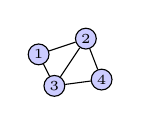
\begin{tikzpicture}[scale=0.4, every node/.style={circle, fill=blue!20, draw, inner sep=1pt, font=\tiny}]
                    \node (A) at (0,1) {1};
                    \node (B) at (1.5,1.5) {2};
                    \node (C) at (0.5,0) {3};
                    \node (D) at (2,0.2) {4};
                    \draw (A) -- (B); \draw (A) -- (C); \draw (B) -- (C); \draw (B) -- (D); \draw (C) -- (D);
                \end{tikzpicture} \\
                \tiny Graphe hybride ($\alpha$)
            \end{block}
        \end{column}
        
        \begin{column}{0.04\textwidth}
            \centering $\rightarrow$
        \end{column}

        \begin{column}{0.20\textwidth}
            \begin{block}{\centering \scriptsize 2. Métriques}
                \scriptsize \centering \vspace{0.1cm}
                Calcul des métriques : Louvain, Infomap, Node2vec, Adamic-Adar, etc.
                \vspace{0.25cm}
            \end{block}
        \end{column}

        \begin{column}{0.04\textwidth}
            \centering $\rightarrow$
        \end{column}

        \begin{column}{0.20\textwidth}
            \begin{exampleblock}{\centering \scriptsize 3. Modèle}
                \scriptsize \centering \vspace{0.1cm}
                \textbf{XGBoost} \\
                Entraînement à la prédiction de liens.
            \end{exampleblock}
        \end{column}

        \begin{column}{0.04\textwidth}
            \centering $\rightarrow$
        \end{column}

        \begin{column}{0.20\textwidth}
            \begin{alertblock}{\centering \scriptsize 4. SHAP}
                \scriptsize \centering \vspace{0.05cm}
                Calcul des SHAP valeurs $\phi_i$ de chaque métrique. \\
                \tiny Additivité : $\phi_{i+j} = \phi_i + \phi_j$
            \vspace{0.05cm}
            \end{alertblock}
        \end{column}
    \end{columns}

    \vspace{0.3cm}
    \hrule
    \vspace{0.2cm}

    \textbf{Protocole anti-leakage} : pour éviter toute fuite d'information lors du calcul des métriques.
    \begin{enumerate}
        \item \textbf{Évaluation Externe (10\,\% des liens) :} Extrait dès le départ. Dataset constitué de métriques calculées sur le graphe restant (90\,\%). Ratio $1:51$ non-liens. $\rightarrow$ Strictement mis de côté pour la mesure finale.
        \item \textbf{Validation Interne (15\,\% des liens) :} Sert de cible pour l'entrainement de XGBoost. Dataset consitué de métriques calculées sur le graphe restant (75\,\%). Ratio $1:11$ non-liens.
        \item \textbf{k-fold cross-validation :} Optimisation des hyperparamètres effectué sur le graphe privé des liens d'évaluation externe (90\,\% des liens).
    \end{enumerate}

\end{frame}

% Slide 11 : Validation du modèle sur les Ground Truth
\begin{frame}{Validation du Framework sur les vérités de terrain}
    \begin{itemize}
        \item \textbf{Objectif :} Prouver l'efficacité du duo XGBoost + SHAP.
        \item \textbf{Procédé :} Entrainement de \textit{XGBoost} avec uniquement \texttt{GT\_pos} (distance exacte) et \texttt{GT\_sbm} (densité de bloc).
        \begin{center}
            % On ajuste la hauteur pour que l'image tienne bien dans la slide Madrid
            \includegraphics[height=5cm, keepaspectratio]{20 SHAPvals_GT_evolution_sbmv4.png}
        \end{center}
        \item \textbf{Conclusion :} Les SHAP valeurs finales semblent fiables, et valider le fonctionnement du modèle.
    \end{itemize}
\end{frame}

% Slide 12 : Résultats par paradigme (∑)
\begin{frame}{Analyse SHAP sur 22 métriques Topologiques, Communautaires, ou Embeddings}
    \begin{center}
            \includegraphics[height=6cm, keepaspectratio]{201 SHAPvals_top10_heatmap_sbmv4.png}
    \end{center}
        
    \vspace{-0.3cm}
    \begin{itemize}
        \item \textbf{Effet d'extinction} induit par les coupures de XGBoost et l'approximation de \textit{TreeSHAP} 
    \end{itemize}
\end{frame}

% Slide 13 : Polyvalence géométrico-structurelle des métriques
\begin{frame}{Polyvalence géométrico-structurelle des métriques}
    \begin{center}
            \includegraphics[height=6cm, keepaspectratio]{204bis 00_perfs_AllMetrics_artificial_graph_sbmv_4_10iter_20260527s_AUC-ROC_eval_CI99_SBM_ratio.png}
    \end{center}

    \textbf{Remarque :} les métriques Communautaires et issues d'Embeddings performent aussi bien sur les graphes spatiaux que géométriques purs.
\end{frame}

% Slide 14 : Corrélation avec la GT
\begin{frame}{Corrélations entre les features et les \textit{Ground Truth} géométriques et communautaires}
    \vspace{-0.6cm}
    \begin{center}
        
\includegraphics[height=5.3cm, keepaspectratio]{206 00_Correl_individual_features_VS_GT_comparison.png}
    \end{center}
    \begin{block}{\small Conclusion 1 :  Les métriques \textbf{Communautaires} et d'\textbf{Embedding} semblent flexibles :}
        \begin{itemize}
            \scriptsize
            \item Elles capturent le signal géométrique ($\text{GT}_{\text{pos}}$) lorsque la structure est majoritairement spatiale ($\alpha < 0.5$).
            \item Elles convergent vers le signal de bloc ($\text{GT}_{\text{sbm}}$) en régime majoriatirement communautaire ($\alpha > 0.5$).
        \end{itemize}
    \end{block}
\end{frame}

% Slide 15 : Quantification de la colinéarité
\begin{frame}{Colinéarité inter-groupe}
    \small Mesure de la corrélation de Spearman moyenne entre les caractéristiques communautaires et géométriques :
    
    \begin{table}[!ht]
        \centering
        \begin{tabular}{cc}
            \hline
            \textbf{Ratio SBM ($\alpha$)} & \textbf{Corrélation Moyenne Inter-Groupe $|\rho| \pm \text{IC}_{95\%}$} \\
            \hline
            1,0 & 0,6166 $\pm$ 0,0210 \\
            0,9 & 0,5392 $\pm$ 0,0205 \\
            0,8 & 0,4409 $\pm$ 0,0143 \\
            0,7 & 0,3993 $\pm$ 0,0068 \\
            0,6 & 0,3403 $\pm$ 0,0111 \\
            0,5 & 0,3133 $\pm$ 0,0072 \\
            0,4 & 0,3978 $\pm$ 0,0125 \\
            0,3 & 0,4535 $\pm$ 0,0250 \\
            0,2 & 0,5157 $\pm$ 0,0182 \\
            0,1 & 0,5768 $\pm$ 0,0134 \\
            0,0 & 0,6330 $\pm$ 0,0184 \\
            \hline
        \end{tabular}
    \end{table}

    \begin{block}{\small Conclusion 2 :  Elles capturent partiellement les mêmes informations :}
        \begin{itemize}
            \scriptsize
            \item Particulièrement marqué sur les graphes purs ($ \alpha \to 0 \enspace \text{ou} \enspace \alpha \to 1 $)
            \item Cette redondance informationnelle explique leur faible complémentarité.
        \end{itemize}
    \end{block}
\end{frame}


\section{Décorrélation, méthode 1 : Louvain débiaisé}
% --- Slide de transition 16 ---
{
\setbeamercolor{background canvas}{bg=structure.fg}
\begin{frame}[plain] % [plain] enlève le header et le footer
    \centering
    \vfill
    \Huge \bfseries \textcolor{white}{4. et 5. Décorrélation, proposition de 2 méthodes : Louvain débiaisé \& SiNE débiaisé}
    \vfill
\end{frame}
}

% Slide 17 : Méthode 1 : Louvain spatialement décorrélé
\begin{frame}{méthode 1 : Louvain spatialement décorrélé}
    \begin{itemize}
        \item \textbf{Idée :} Remplacer le modèle nul de configuration classique (Newman-Girvan) utilisé nativement par Louvain, qui ignore l'espace.
        \item \textbf{Étape 1 : Inférence d'un modèle nul gravitaire Degré-Corrigé}, par optimisation alternée de $\alpha$ par descente de coordonnées et de $\beta$ par maximum de vraisemblance :
        $$P_{uv} = \frac{1}{1 + e^{-(\alpha_u + \alpha_v - \beta \cdot d_{uv})}}$$
        \item \textbf{Étape 2 : Injection dans le calcul de modularité de Louvain} (via \texttt{MetaLouvain})
        $\rightarrow$ on soustrait l'attente géométrique :
        $$Q_{\text{Spatial}} = \frac{1}{2m} \sum_{u,v} \left( A_{uv} - P_{\text{grav-DC}} \right) \mathbb{I}(b_u = b_v)$$
        \item \textbf{Étape  3 : Inférence de communautés Louvain} sans autres modifications.
    \end{itemize}s
\end{frame}

% Slide 18 : Validation de la décorrélation, via l'Information Mutuelle
\begin{frame}{Validation de l'indépendance informationnelle via l'Information Mutuelle}
    \begin{itemize}
        \item \textbf{Objectif :} Prouver l'efficacité du débiaisage
        \item \textbf{Procédé :} Etude de l'Information Mutuelle Ajustée (AMI) entre la métrique et la \texttt{GT\_pos}.
        \begin{center}
            \includegraphics[height=4.2cm, keepaspectratio]{208bis 02_MI_adjusted_louvain_vs_spatialLouvain.png}
        \end{center}
        \item \textbf{Conclusion :} Décorrélation flagrante avec \texttt{GT\_pos}, et même léger gain avec \texttt{GT\_sbm} pour $0.2 \leq \alpha \leq 0.5$ 
    \end{itemize}
\end{frame}

% Slide 19 : Résultats empiriques de Louvain Décorrélé
\begin{frame}{Performances empiriques en prédiction de lien}
    \vspace{-0.25cm}
    \begin{itemize}
        \item \textbf{Méthode :} Comparaison des performances de \texttt{XGBoosts} entraînés avec \{\texttt{GT\_sbm}; \texttt{louvain standard}\}, et  avec \{\texttt{GT\_sbm};\texttt{louvain décorrélé}\}.
    \end{itemize}

    \vspace{0.2cm}

    \begin{columns}[b] % Alignement par le bas pour caler les légendes
        \begin{column}{0.48\textwidth}
            \centering
            \includegraphics[width=\textwidth]{209bis 01_artificial_graphs_shuffled_v4_comuAndEmb_30iter_GTposAndComu_20260529_AUC-ROC_eval_CI99_SBM_ratio.png}
            
            \vspace{0.1cm}
            {\footnotesize (a) Louvain Standard vs Décorrelé\\(somme pondérée)}
        \end{column}
        
        \hfill
        
        \begin{column}{0.48\textwidth}
            \centering
            \includegraphics[width=\textwidth]{211bis 01_artificial_graphs_shuffled_v6_comuAndEmb_30iter_GTposAndComu_20260529_AUC-ROC_eval_CI99_SBM_ratio.png}
            
            \vspace{0.1cm}
            {\footnotesize (b) Louvain Standard vs Décorrelé\\(méthode exposant)}
        \end{column}
    \end{columns}
    
    \begin{center}
        \scriptsize \textit{Les intervalles de confiance à 95\% sont calculés sur 30 itérations.}
    \end{center}

    \vspace{-0.2cm}
    \begin{block}{\small Légers gains autour de $\alpha = 0.5$:}
        \begin{itemize}
            \scriptsize
            \item Visibles sur une plus grande plage ($0.3 \leq \alpha \leq 0.7$) sur graphes contrastés (méthode exposant)
            \item Intuition : limite des inférences de communautés qui ont besoin d'un signal assez fort (cf nombre de communautés)
        \end{itemize}
    \end{block}
\end{frame}

\section{Décorrélation, méthode 2 : SiNE débiaisé }

% Slide 20 : La notion de matrice de résidus continuous
\begin{frame}{méthode 2 : SiNE décorrélé}
    \begin{itemize}
        \item \textbf{Objectif :} inférer des embeddings plutôt que des communautés, plus suceptibles de capturer des signaux faibles.
        \item \textbf{Méthode :} les inférer sur la \textbf{matrice de résidus} $R = A - P_{\text{grav-DC}}$
        \item \textbf{Problématique :} Comment calculer des embeddings sur un graphe réiduel signé et très dense ?
    \end{itemize}
    \begin{block}{Solution pour la densité :}
        \begin{itemize}
            \item échantillonage stochastique par softmax (noté $S$), pour tout noeud $i$, parmi son ensemble de voisins $\mathcal{V}_i$:
            $ \quad  p(j \mid i) = \frac{e^{|R_{ij}| / T}}{\sum_{w \in \mathcal{V}_i} e^{|R_{iw}| / T}}$
        \end{itemize}
    \end{block}
    \begin{block}{Solution pour le signe : perte antagoniste}
        \begin{itemize}
            \item si $R_{uv} > 0$, on encourage le rapprochement
            \item si $R_{uv} < 0$, on encourage un espacement suppérieur à une marge $m$.
        \end{itemize}
        $$ \mathcal{L} = \mathbb{E}_{(u,v) \sim \mathcal{S}} \left[ \mathbb{I}(R_{uv} \ge 0) \|\mathbf{z}_u - \mathbf{z}_v\|_2 + \mathbb{I}(R_{uv} < 0) \max\left(0, m - \|\mathbf{z}_u - \mathbf{z}_v\|_2\right) \right] $$
        
    \end{block}
\end{frame}

% Slide 21 : Validation de l'indépendance informationnelle via l'AMI
\begin{frame}{Validation de l'indépendance informationnelle via l'AMI}
    \begin{center}
        \includegraphics[height=4.2cm, keepaspectratio]{208ter 02_MI_adjusted_deepwalk_vs_spatialSine.png}
    \end{center}
    \begin{itemize}
        \item \textbf{Conclusion :} Décorrélation flagrante avec \texttt{GT\_pos} (mais imparfaite pour $\alpha \leq 0.1$), sans gain avec \texttt{GT\_sbm}
    \end{itemize}
\end{frame}

% Slide 22 : Résultats empiriques de SiNE Décorrélé
\begin{frame}{Performances empiriques en prédiction de lien}
    \vspace{-0.25cm}
    \begin{itemize}
        \item \textbf{Méthode :} Comparaison des performances de \texttt{XGBoosts} entraînés avec \{\texttt{GT\_sbm}; \texttt{louvain standard}\}, et  avec \{\texttt{GT\_sbm};\texttt{louvain décorrélé}\}.
    \end{itemize}

    \vspace{0.2cm}

    \begin{columns}[b] % Alignement par le bas pour caler les légendes
        \begin{column}{0.48\textwidth}
            \centering
            \includegraphics[width=\textwidth]{210bis 01_artificial_graphs_shuffled_v4_comuAndEmb_30iter_GTposAndSine_20260529_AUC-ROC_eval_CI99_SBM_ratio.png}
        
            \vspace{0.1cm}
            {\footnotesize (a) DeepWalk vs SiNE Décorrelé\\(somme pondérée)}
        \end{column}
        
        \hfill
        
        \begin{column}{0.48\textwidth}
            \centering
            \includegraphics[width=\textwidth]{212bis 01_artificial_graphs_shuffled_v6_comuAndEmb_30iter_GTposAndSine_20260529_AUC-ROC_eval_CI99_SBM_ratio.png}
            
            \vspace{0.1cm}
            {\footnotesize (b) DeepWalk vs SiNE Décorrelé\\(méthode exposant)}
        \end{column}
    \end{columns}
    
    \begin{center}
        \scriptsize \textit{Les intervalles de confiance à 95\% sont calculés sur 30 itérations.}
    \end{center}

    \vspace{-0.2cm}
    \begin{block}{\small Gains sur une plage plus importante de $\alpha$ :}
        \begin{itemize}
            \scriptsize
            \item dès la méthode par somme pondérée, indiquant une meilleure sensibilité
            \item \textbf{remarque :} la surperformance pour $\alpha = 1$ semble indiquer que la méthode est légèrement plus efficace que DeepWalk mêm sans l'aspect débiasage.
            \item \textbf{limite :} comparaison avec DeepWalk, pas d'équivalent strict sans débiaisage.
        \end{itemize}
    \end{block}
\end{frame}

\section{Conclusion et Perspectives}

% Slide 23 : Conclusion Générale
\begin{frame}{Conclusion et Perspectives}
    \begin{block}{Synthèse des travaux}
        \begin{itemize}
            \item Preuve conceptuelle de la colinéarité des métriques de l'état de l'art via le framework XGBoost+SHAP.
            \item Résultats encourageants du débiaisage par modèle nul pour l'inférence de communautés (Louvain spatial) et d'embeddings ($\text{SiNEcustom}$).
        \end{itemize}
    \end{block}
    \begin{block}{Perspectives de recherche et limites}
        \begin{itemize}
            \item \textbf{Benchmark réel :} confronter ces méthodes à un benchmark de graphes réels.
            \item \textbf{Modèles nuls :} Explorer l'utilisation d'autres modèles nuls :
                \begin{itemize}
                    \item autres modèles spatiaux (radiation, ...)
                    \item modèles capturant d'autres informations : temporelle, communautés, nouveaux modèles nuls à potentiellement développer.
                \end{itemize}
            \item \textbf{Optimisation algorithmique:} Implémentation optimisée des méthodes proposées nécessaire au passage à l'échelle.
        \end{itemize}
    \end{block}
\end{frame}

% --- Slide FINALE 24 ---
{
\setbeamercolor{background canvas}{bg=structure.fg}
\begin{frame}[plain] % [plain] enlève le header et le footer
    \centering
    \vfill
    \Huge \bfseries \textcolor{white}{Place à vos questions}
    \vfill
\end{frame}
}

\end{document}